\chapter{Introduction}
\label{ch:introduccion}

\section{Motivation}

The web provides a vast amount of information, including a lot of text, but it is increasingly dominated by visual information, both static (pictures) and dynamic (videos).  However, much of that visual information is not accessible to those with visual impairments, or with slow internet speeds that prohibit the loading of images. Image captions, manually added by content providers (typically by using the \textit{ Alt-text} HTML tag), is one way to make this content more accessible, so that a \textit{text-to-speech} system can be applied to generate a natural-language description of images and videos. However, existing human-curated image descriptions are added for only a very small fraction of web images. Thus, there is great interest in developing methods to automatically generate image descriptions.

Automatic image description --also known as automatic image captioning-- can be defined as the task of automatically generating a description of an image using natural language. It is a very challenging problem that encompasses two kind of problems: the problem of understanding an image, which is a \textbf{Computer Vision (CV)} task, and the problem of generating a meaningful and grammatically-correct description of the image, which is a kind of \textbf{Natural-Language Processing (NLP)} task . Therefore, to tackle this task it is necessary to advance the research in the two fields, CV and NLP, as well as promoting the cooperation of both communities to address the specific problems arising when combining both tasks.

\Cref{fig:image-captioning} shows an example of the automatic image generation tasks addressed by this project.

\begin{figure}[hpt]
	\centering
	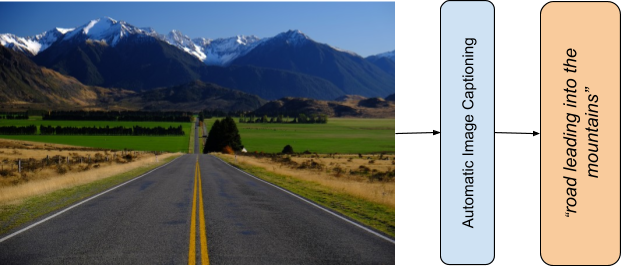
\includegraphics[scale=0.5]{/ch1/image-captioning.png}
	\caption{Image captioning can help millions with visual impairments by converting images captions to text. Image by \href{https://www.flickr.com/photos/francisvallance/}{Francis Vallance (Heritage Warrior)}, used under \href{https://creativecommons.org/licenses/by/2.0/}{CC BY 2.0 license}.}
	\label{fig:image-captioning}
\end{figure}

In addition to the aforementioned application of image captioning to help the visually impaired, there are many other use cases in which automatic image descriptions may help. Generally speaking, any domain in which images need to be interpreted by humans, but human availability is scarce, or the task at hand is tedious, may surely benefit from algorithms able to automatically generate textual image descriptions.

A vast area of application is that of \textbf{Concept-Based Image Retrieval}. This kind of task, also named as "description-based" or "text-based" image indexing/retrieval, refers to retrieval from text-based indexing of images that may employ keywords, subject headings, captions, or natural language text. The main problem with this approach to image retrieval is the scarcity of image descriptions, since having humans manually annotate images by entering keywords or descriptions in a large database can be very tedious and time consuming \footnote{This is one of the reasons explaining the upswing of \textit{Content-Based Image Retrieval}, which uses content derived from the visual properties of the image, like color, textures and shape, instead of semantic and descriptive data such as keywords and captions}.  Therefore, automatic image description may be of great utility, and it can be applied to many areas requiring image indexing and retrieval, such as biomedicine, education, digital libraries, etc., as well as general web search. In addition to automate the annotation of images, there is an extra benefit in using captions vs keywords: image captions are semantically richer and more sophisticated, thus allowing for more complex queries to improve the precision of the search.

Another area where automatic image captioning may be of great utility is the analysis and extraction of information from videos. Some video monitoring tasks are very boring and tedious. An automated mechanism to describe scenes in video footage will be of great utility for creating summaries or monitoring specific situations and events. \footnote{As an interesting example, Shell is conducting a pilot study using deep-learning to automatically monitor video footage in order to identify safety hazards and generate alerts (\href{https://customers.microsoft.com/en-us/story/shell-mining-oil-gas-azure-databricks}{link})}.

Automatic image description can also be used to improve image indexing with, since they provide a more sophisticated and semantically rich description that image classification or simple image tagging. This kind of semantic indexes would be very very useful for any kind of Content-Based Image Retrieval application, which would help improve any king of Content-Based Image Retrieval. This kind of Having images automatically generated captions for images that originally hasn't been described, would help finding images based on a complex description rather that a simple collection of tags. This is some

\section{Goals}

This project aims at advancing in the task of automatically generating image descriptions. That is the ultimate goal of the project. However, in order to achieve such an abstract goal, we decompose it into various subgoals, as follows:

\begin{enumerate}
\item Get a solid understanding of the problem at hand and review the state-of-art solutions to it
\item Get practical knowledge on the technologies required to solve this problem
\item Develop a model using a benchmark dataset like the Flickr30K
\item Scale the model to a larger benchmark dataset such as the COCO\cite{Lin2014} dataset or the more recent Conceptual Captions Dataset by Google \cite{Sharma2018}  (see \cref{fig:conceptual-captions}).
\item Evaluate the model, ideally partaking in some challenge or competition, like the ones using the COCO dataset or the Conceptual Captions dataset.
\end{enumerate}

\begin{figure}[hpt]
	\centering
	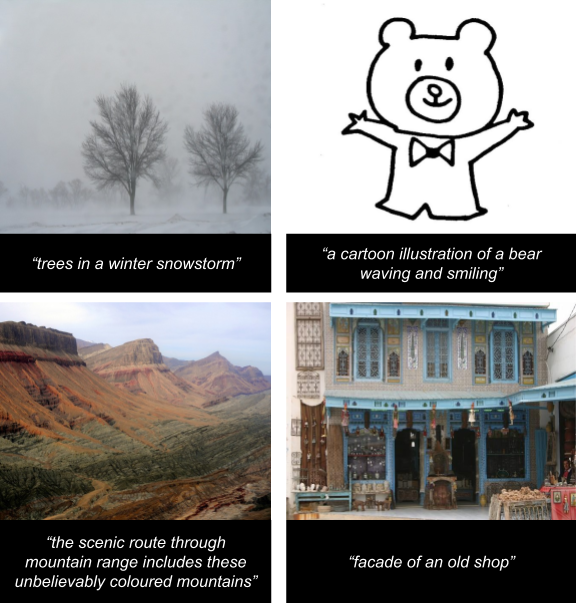
\includegraphics[scale=0.5]{ch1/conceptual-captions-example.png}
	\caption{Illustration of images and captions in the Conceptual Captions dataset.Clockwise from top left, images by Jonny Hunter, SigNote Cloud, Tony Hisgett, ResoluteSupportMedia. All images used under \href{https://creativecommons.org/licenses/by/2.0/}{CC BY 2.0 license}.}
	\label{fig:conceptual-captions}
\end{figure}

\section{Methodology}

This project is mainly an academical, research-oriented project, so it would follow a process model which is common for these kind of projects, for instance, it will include a comparatively long review of the state of the art, as well as a public defense at the end. However, this project will also include the development of a software artifact to solve a data-analytic problem, therefore we should benefit from using a data-analytic model as the well known and widely adopted \textbf{CRISP-DM}. CRISP-DM, which stands for \textit{Cross-Industry Standard Process for Data Mining}, is an open standard process model and an industry-proven methodology to guide data mining projects.

As a methodology, it includes descriptions of the typical phases of a project, the tasks involved with each phase, and an explanation of the relationships between these tasks.

As a process model, CRISP-DM provides an overview of the data mining life cycle.

\Cref{fig:crisp-dm} depicts the relationships between the different phases of the CRISP-DM model. The sequence of the phases is not strict and moving back and forth between different phases is often required. The arrows in the process diagram indicate the most important and frequent dependencies between phases. The outer circle in the diagram symbolizes the cyclic nature of data mining itself. A data mining process continues after a solution has been deployed. The lessons learned during the process can trigger new, often more focused business questions, and subsequent data mining processes will benefit from the experiences of previous ones.

\begin{figure}[hpt]
	\centering
	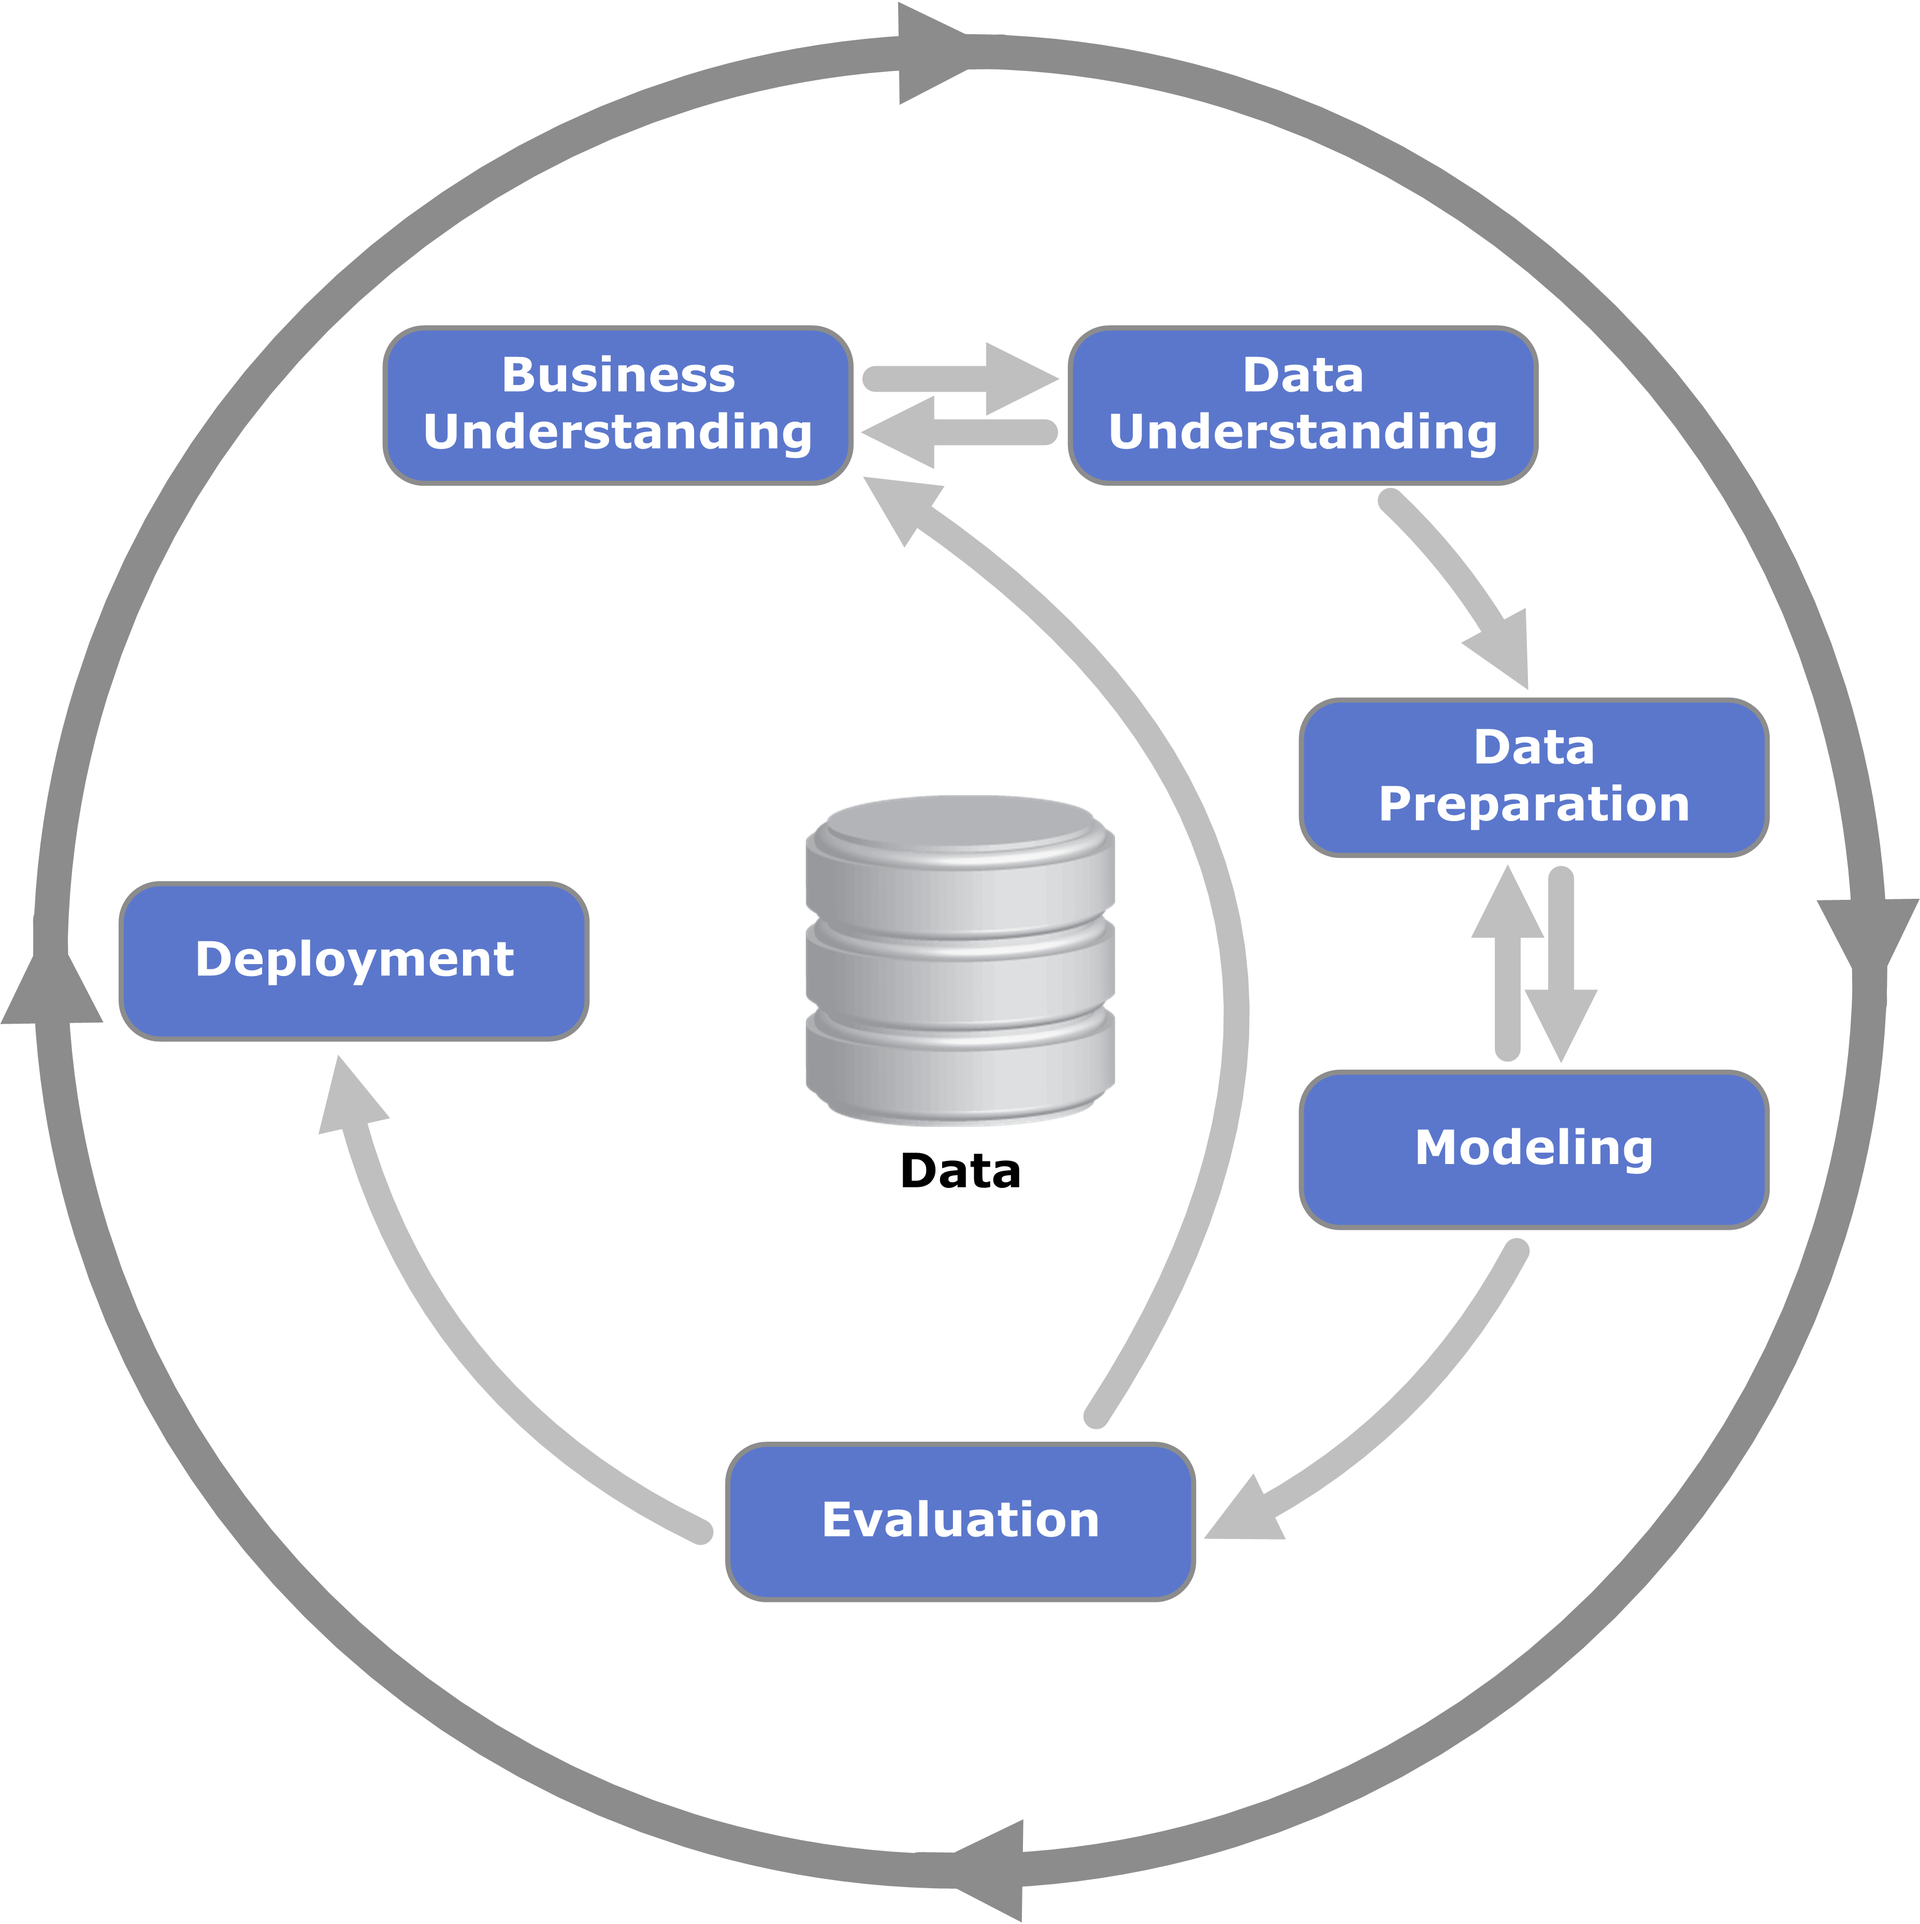
\includegraphics[scale=0.25]{ch1/crisp-dm.png}
	\caption{Process diagram showing the relationship between the different phases of CRISP-DM. Image by Kenneth Jensen, used under \href{https://creativecommons.org/licenses/by/2.0/}{CC BY-SA 3.0 license..}}
	\label{fig:crisp-dm}
\end{figure}

The process model consists of six major phases:

\begin{itemize}
\item \textbf{Business Understanding}: Includes an in-depth analysis of the business objectives and needs. The situation is assessed and the goals of the project are defined. This should follow the setting up of a plan to proceed.
\item \textbf{Data Understanding}: Conduct initial or exploratory data analysis to become familiar with data and identify potential problems. Examine properties of data and verify its quality by answering questions concerning the completeness and accuracy of the data.
\item \textbf{Data Preparation}: After the data sources are completely identified, proper selection, cleansing, constructing and formatting should be done before modelling. 
\item \textbf{Modeling}: Modeling is usually conducted in multiple iterations, which involve running  several models using the default parameters and then fine-tune the parameters or revert to the data preparation phase for additional preparation. Usually, there are different ways to look at a given problem, so it is convenient to build multiple models,
\item \textbf{Evaluation}: The results of models are evaluated in the backdrop of business intentions. New objectives may sprout up owing to the new patterns discovered. This is, in fact, an iterative process, and the decision whether to consider them or not has to be made in this step before moving on to the final phase
\item \textbf{Publication}. The final information gathered has to be presented in a usable manner to the stakeholders.  This has to be done as per their expectations and business requirements.
\end{itemize}


\section{Planning}

This section briefly describes the planning for this Final Master's work.

\begin{table}[ht]
\centering
\caption{Main tasks and milestones.}
\label{tab:retrieval-classification}
\begin{tabular}[t]{lll}
    \toprule
    Phase & End  & Description\\
    \midrule
    1 & 3/3/2019 & Definition and planning\\
    2 & 24/3/2019 & State of the Art\\
    3 & 19/5/2019 & Development\\
    4 & 9/6/2019 & Complete this report\\
    5 & 16/6/2019 & Presentation\\
    \bottomrule
\end{tabular}
\end{table}


Phase 2 will encompass the following tasks:
\begin{itemize}
\item Reviewing relevant bibliography
\item Studying the problem domain (business understanding), and becoming familiar with the data. At this stage we would also start preparing the data for the modeling stage
\end{itemize}

Phase 3 will be the longest phase, and it will include the following tasks:
\begin{itemize}
\item Preparing the data. Although data preparation could be started during phase 2, depending on the chosen models it could be necessary to conduct some additional data preparation operations
\item Generating one or various models. We plan at creating at least two models, one that would replicate existing work, and another one to explore new ideas and try to beat the baseline model.
\item Evaluating the models, and very specifically, compare our model against the replicated model.
\item Publication: We consider two courses of action: a) participating in the Conceptual Captions Challenge by Google, and b) delivering some product to the final user, although it would be a very basic prototype given the little time available.
\end{itemize}

In phase 4 we will complete this report. This phase would probably overlap with some of the tasks in phase 3 that will require additional time, like the evaluation of the models and the participation in challenges.

In phase 5 we will present the results achieved for its evaluation. These results will benchmark results, documentations, and the code itself. Finally, there will be a public defense of the project in front of an academic board, which should be conveniently prepared.

